\documentclass[sigconf]{acmart}

\usepackage[utf8]{inputenc}
% \usepackage[hyphens]{url}
% \usepackage[pdftex,urlcolor=black,colorlinks=true,linkcolor=black,citecolor=black]{hyperref}
% \def\sectionautorefname{Section}
% \def\subsectionautorefname{Subsection}

\usepackage{graphicx}
\usepackage[export]{adjustbox}
\usepackage{caption}
\usepackage{subcaption}
\usepackage{textcomp}
\usepackage{gensymb}
\usepackage[super]{nth}

\usepackage{listings}
\usepackage{color}
\definecolor{lightgray}{rgb}{.9,.9,.9}
\definecolor{darkgray}{rgb}{.4,.4,.4}
\definecolor{purple}{rgb}{0.65, 0.12, 0.82}

\lstdefinelanguage{JavaScript}{
  keywords={typeof, new, true, false, catch, function, return, null, then, catch, switch, var, const, let, if, in, while, do, else, case, break},
  keywordstyle=\color{blue}\bfseries,
  ndkeywords={class, export, boolean, throw, implements, import, this},
  ndkeywordstyle=\color{darkgray}\bfseries,
  identifierstyle=\color{black},
  sensitive=false,
  comment=[l]{//},
  morecomment=[s]{/*}{*/},
  commentstyle=\color{purple}\ttfamily,
  stringstyle=\color{red}\ttfamily,
  morestring=[b]',
  morestring=[b]"
}

\lstset{
   language=JavaScript,
   extendedchars=true,
   basicstyle=\footnotesize\ttfamily,
   showstringspaces=false,
   showspaces=false,
   numberstyle=\footnotesize,
   numbersep=9pt,
   tabsize=2,
   frame = single,
   breaklines=true,
   showtabs=false,
   captionpos=b
}

% todo macro
\usepackage{color}
\newcommand{\todo}[1]{\noindent\textcolor{red}{{\bf \{TODO}: #1{\bf \}}}}

\settopmatter{printacmref=false}

% Copyright
%\setcopyright{none}
%\setcopyright{acmcopyright}
%\setcopyright{acmlicensed}
\setcopyright{rightsretained}
%\setcopyright{usgov}
%\setcopyright{usgovmixed}
%\setcopyright{cagov}
%\setcopyright{cagovmixed}


% DOI
\acmDOI{10.475/123_4}

% ISBN
\acmISBN{123-4567-24-567/08/06}

%Conference
\acmConference[WOODSTOCK'97]{ACM Woodstock conference}{July 1997}{El
  Paso, Texas USA}
\acmYear{1997}
\copyrightyear{2016}

\acmArticle{4}
\acmPrice{15.00}

% These commands are optional
%\acmBooktitle{Transactions of the ACM Woodstock conference}
%\ editor{Jennifer B. Sartor}
% \editor{Theo D'Hondt}
% \editor{Wolfgang De Meuter}


\begin{document}
\title[What is in a~Web View?]{What is in a~Web View?
An Analysis of Progressive Web App Features
When the Means of Web Access is not a~Web Browser}  

% \titlenote{}
% \subtitle{}
% \subtitlenote{}


\author{Thomas Steiner}
% \authornote{}
% \orcid{1234-5678-9012}
\affiliation{%
  \institution{Google Germany GmbH}
  \streetaddress{ABC-Straße 19}
  \city{20354 Hamburg}
  \country{Germany}
}
\email{tomac@google.com}

%\author{Michael Yeung}
%% \authornote{}
%% \orcid{1234-5678-9012}
%\affiliation{%
%  \institution{Google Hong Kong}
%  \streetaddress{1~Matheson Street}
%  \city{Causeway Bay}
%  \country{Hong Kong}
%}
%\email{micyeung@google.com}

% The default list of authors is too long for headers.
%\renewcommand{\shortauthors}{B. Trovato et al.}

\begin{abstract}
Progressive Web Apps (\textsc{pwa}) are a~new class of Web applications,
enabled for the most part by the Service Workers \textsc{api}s.
Service Workers allow apps to \emph{work offline}
by intercepting network requests to deliver programmatic or cached responses,
Service Workers can receive \emph{push notifications}
and \emph{synchronize} data in the background
even when the app is not running,
and---together with Web App Manifests---allow users to \emph{install \textsc{pwa}s}
to their devices' home screens.
Service Workers being a Web standard, support has landed in several
stand-alone Android Web browsers---among them (but not limited to)
Chrome and its open-source foundation Chromium, Firefox, Edge, Opera,
\textsc{uc}~Browser, Samsung Internet, and---eagerly awaited---i\textsc{os} Safari.
In this paper, we examine the \textsc{pwa} feature support situation in \emph{Web Views},
that is,\ \emph{in-app Web experiences} that are explicitly \emph{not} stand-alone browsers.
Such in-app browsers can commonly be encountered in chat applications like WeChat or WhatsApp,
online social networks like Facebook or Twitter, but also email clients like Gmail,
or simply anywhere where Web content is displayed inside native apps.
We have developed an open-source application called \emph{\textsc{pwa} Feature Detector}
that allows for easily testing in-app browsers (and naturally stand-alone browsers as well),
and have evaluated the level of support for \textsc{pwa} features
on different devices and Web Views.
On the one hand, our results show that there are big differences
between the various Web View technologies
and the browser engines they are based upon,
but on the other hand, that the results
are independent from the devices' operating systems,
which is good news given the problematic update policy of many device manufacturers.
These findings help developers make educated choices when it comes to determining
whether a~\textsc{pwa} is the right approach given their target users' means of Web access.
\end{abstract}

%
% The code below should be generated by the tool at
% http://dl.acm.org/ccs.cfm
% Please copy and paste the code instead of the example below.
%

\keywords{Progressive Web Apps, Service Workers, Web Views}

\maketitle

\section{Introduction}

In recent years, there has been a~paradigm shift
from browser to native apps and back to browser again.
The Web currently is undergoing a silent revolution with Web apps,
more descriptively \emph{Progressive Web Apps},
or for short just \textsc{pwa}s.
How did we get there?

\subsection{History of Progressive Web Apps}

Since around 2005, Web development has moved from static multi-page \emph{documents}
to single-page \emph{applications}, heavily enabled by the \texttt{XMLHttpRequest} \textsc{api},
a~process that eventually led Garrett to coin the term \emph{Ajax}
(Asynchronous JavaScript and XML~\cite{garret2005ajax}) to describe this shift.
Despite an early push for Web-based apps on devices such as the 2007 iPhone,
attempts at Web apps mostly failed by comparison to native apps
that are distributed through app stores rather than the Web.
Native apps not only had direct hardware access to, \emph{e.g.},\ camera and microphone,
to various sensors like accelerometer or geolocation, but also just in general provided
a~better user experience and booted faster, compared to having to load in a~browser at runtime.
Additionally, advanced offline support and push notifications were simply unthinkable
for Web applications of the epoch, and Web app icons
that already could be added to devices' home screens
were mostly just bookmarks with---apart from full screen mode---no special behavior.
While straightforward offline scenarios could be realized with
\texttt{AppCache}~\cite{vankesteren2008offlinewebapps}, more complex offline scenarios were error-prone
and hard to get right~\cite{archibald2012douchebag}.

As the Web platform matured and more and more
hardware-related \textsc{api}s were implemented in browsers,
in the end it was the addition of Service Workers~\cite{russell2017serviceworkers}
to the Chromium browser in 2014~\cite{cooney2014chromium} that started to unlock a~new class of Web apps
that finally could \emph{work offline}, receive \emph{push notifications}
and \emph{synchronize} data in the background even when the app was not running,
and---together with Web App Manifests~\cite{caceres2017manifest}---allowed
users to actually \emph{install \textsc{pwa}s} to their devices' home screens
with proper operating system integration~\cite{kinlan2017a2hs}.
Other Android browsers like Mozilla Firefox, Microsoft Edge, Opera, \textsc{uc}~Browser, Samsung Internet,
and---eagerly awaited---Apple Safari on i\textsc{os},
as well as several browsers more followed in implementing Service Workers.
Now, even multinational companies like Twitter
or trivago bet on \textsc{pwa}~\cite{gallagher2017twitterlite,twg2017trivago},
as well as giant national players like Tencent News or Sina Weibo in China~\cite{zhu2017pwa}.
\autoref{fig:pwa-features} shows the \textsc{pwa} of Flipkart, a~shopping site popular in India,
running in the Google Chrome browser on Android.

\begin{figure}[hbt]
  \centering
  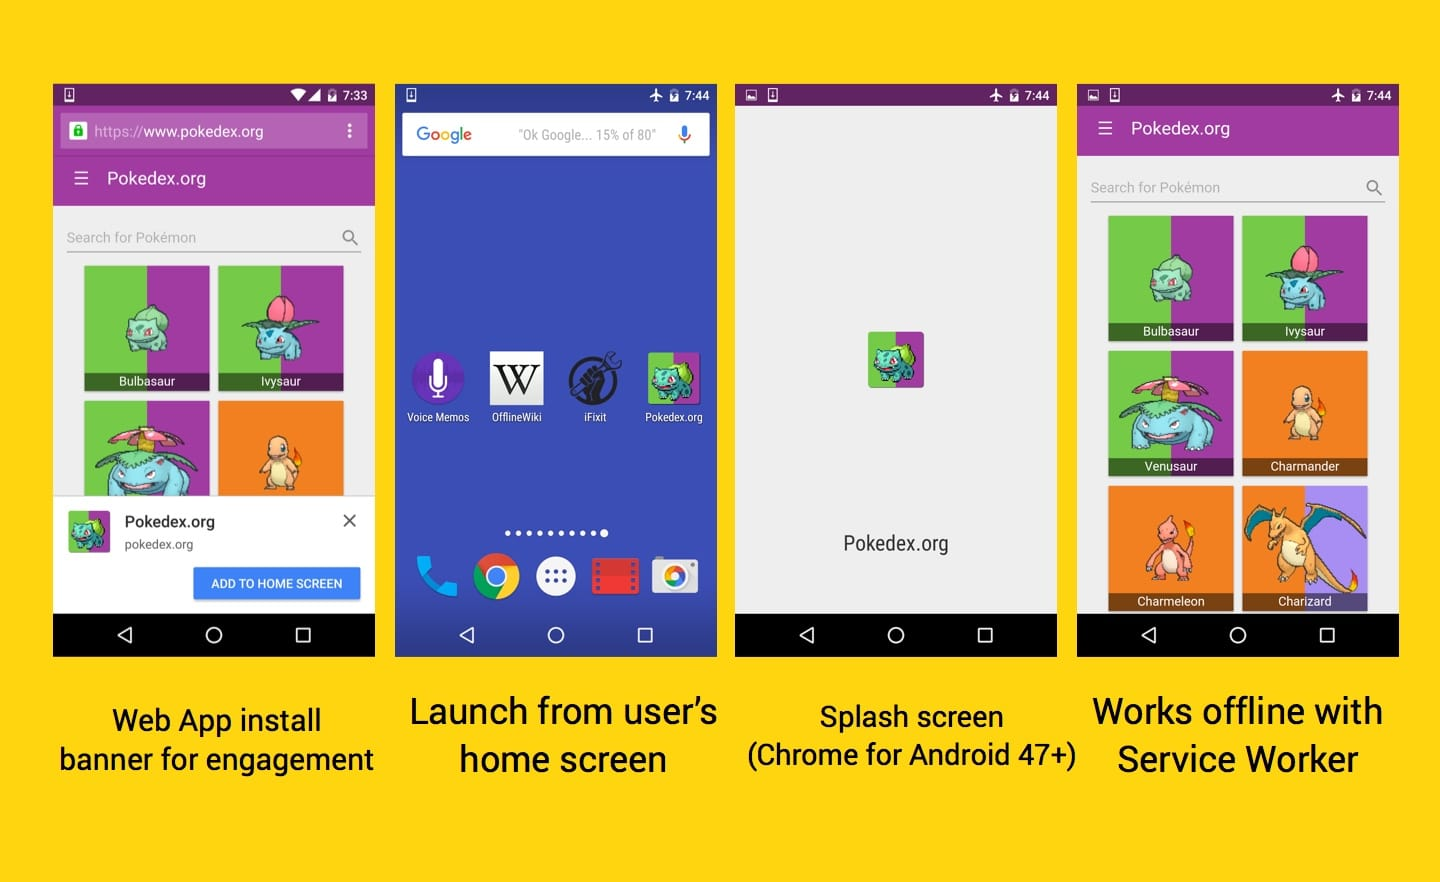
\includegraphics[width=\columnwidth]{pwa-features}
  \caption[Screenshots showing some \textsc{pwa} features]{
    Screenshots showing some \textsc{pwa} features in action
    at the example of Flipkart (\url{https://www.flipkart.com}):
    \emph{(i)}~add to home screen prompt, \emph{(ii)}~icon on the home screen
    \emph{(iii)}~splash screen while launching,
    \emph{(iv)}~launched in full screen without \textsc{url} bar, and
    \emph{(v)}~signaling offline state.}
  \label{fig:pwa-features}
\end{figure}

\subsection{Research Question and Paper Structure}

In this paper, we look at a~special means for accessing \textsc{pwa}s,
namely accessing them explicitly \emph{not} through stand-alone browsers
like the ones listed above,
but through \emph{in-app browsers} that render Web content in the context of native applications.
Examples of such applications with in-app browsers are chat apps like WeChat (Wēixìn) or WhatsApp,
online social networks like Facebook or Twitter, but also email clients like Gmail,
or simply anywhere where Web content is displayed inside native apps.
The technology that these applications leverage internally are so-called \emph{Web Views}.
In order to understand why this presents an interesting research problem,
one needs to first understand the role that applications like WeChat
and thus Web Views play in markets like China.
Chan writes in an article~\cite{chan2015wechat} for the venture capital firm Andreessen Horowitz:
``Millions (note, not just thousands) of lightweight apps live inside WeChat,
much like webpages live on the internet.
\emph{This makes WeChat more like a~browser for mobile websites}, or, arguably,
a~mobile operating system---complete with its own proprietary app store.
The lightweight apps on WeChat are called `official accounts'.
Approved by WeChat after a~brief application process,
there are well over 10~million of these official accounts on the platform---ranging
from celebrities, banks, media outlets, and fashion brands to hospitals, drug stores,
car manufacturers, internet startups, personal blogs, and more''.
Chan goes on: ``WeChat focuses on taking care of the plumbing---overseeing
the integration of such pre-existing services into its portal---by
simply linking users from the wallet menu to webpages from within the app.
It's yet another way in which \emph{WeChat
becomes an integrated browser for the mobile (and web) world}''.
It is to be noted that this development comes to the detriment of the so-called Open Web.
As Yang and Yang write in the Financial Times~\cite{yang2017tencent}:
``[WeChat's] news feed and search tools pull content only from within WeChat's walls
rather than from the open web, including updates posted by individual users called moments,
corporate accounts and an immense collection of WeChat accounts
which are used by newspapers and independent bloggers''.
While personally we do not embrace this development
and are advocates of the open Web,
we nevertheless examine the implications of an in-app closed Web experience
and its impact on \textsc{pwa}s. 

In the remainder of this paper, we first look at the technical background of Web Views
on both Android and i\textsc{os} in \autoref{sec:background}.
We then describe the examined \textsc{pwa} features and their underlying \textsc{api}s
in \autoref{sec:pwa-feature-detector}, in which we also introduce
our application \emph{\textsc{pwa} Feature Detector}.
In continuation, we present and discuss our results in \autoref{sec:results-and-discussion}.
We close the paper with an outlook on future work in \autoref{sec:future-work}
and draw our conclusions in \autoref{sec:conclusions}.

\section{Background on Web Views}
\label{sec:background}

There are several different ways to integrate Web content in native applications,
each having their own benefits and drawbacks.
In the following, we describe the options on the two popular
mobile operating system Android and i\textsc{os}.
While Android had enjoyed Service Worker support for as long as 2014~\cite{cooney2014chromium},
at time of writing (February 2018), Safari on i\textsc{os}
for the first time supported Service Workers
in Beta versions of i\textsc{os}~11.3~\cite{mondello2018safari}.
The implementation is still incomplete and several bugs exist, but in the spirit of
Progressive Enhancement~\cite{champeon2003progressiveenhancement}
the situation is expected to improve over time.

\subsection{Web Views on Android}

\paragraph{Android Web Views with \texttt{WebView}}

In the Android operating system, a~\texttt{WebView}~\cite{android2018webview}
is a~subclass of a~\texttt{View} that displays Web pages.
This class is the basis upon which developers can create their own Web browser
or simply display some online content in their apps.
It does not include any features of a~fully developed Web browser,
such as navigation controls or an address bar.
All that \texttt{WebView} does, by default, is show a~Web page.
Therefore, it uses the system browser's rendering engine to display Web pages
and includes methods to navigate forward and backward through a history,
zoom in and out, perform text searches, inject custom JavaScript, and more.
Looper describes~\cite{looper2015webviews}
the development of the component as follows:
``Whereas earlier versions of the Android \textsc{os}
relied on the WebKit rendering engine to power its \texttt{WebView},
as of Android~4.4, various versions of Chromium are implemented.
Typically, with each consecutive update of Android's~\texttt{os},
a~new version of Chromium would also be included, thereby giving access
to the new rendering engine's capability.
This causes issues in backward compatibility for developers
who must support earlier versions of Android.
To combat this particular problem, as of Android~5.0,
the concept of the auto-updating \texttt{WebView} has been introduced.
Instead of the \texttt{WebView} version and capabilities
depending on Android \textsc{os}' update cycle,
the Android~5.0 \texttt{WebView} is a~system-level \texttt{.apk} file
available in Google Play that can update itself in the background''.

\paragraph{Chrome Custom Tabs with \texttt{CustomTabsIntent}}

While \texttt{WebView}s are completely isolated from the user's regular browsing activities,
Chrome Custom Tabs~\cite{kinlan2016customtabs}, available since Chrome~45 (September 2015)
and instantiatable as \texttt{CustomTabsIntent}, provide a~way for an application
to customize and interact with a~Chrome Activity on Android.
This makes the Web content feel like being a part of the application,
while retaining the full functionality and performance of a~complete Web browser
through a~shared cookie jar and permissions model, so users do not have to log in
to sites they are already connected to, or re-grant permissions they have already granted.

\paragraph{Trusted Web Activity with \texttt{TrustedWebUtils}}

Chrome Custom Tabs solved many issues of Android \texttt{WebView}s,
however, had the drawback of not being available in a~fullscreen variant
without any browser user interface elements like \texttt{WebView}s were.
As of October 2017, Trusted Web Activities~\cite{googledevelopers2017twa} are a~new way to
integrate Web app content such as \textsc{pwa}s with Android apps.
They can be instantiated with the \texttt{TrustedWebUtils}
and use a~communication protocol based on Chrome Custom Tabs.
Content in a~Trusted Web Activity is trusted---the app and the site it opens
are expected to come from the same developer, this is verified using Digital Asset
Links.\footnote{Digital Asset Links:
\url{https://developers.google.com/digital-asset-links/}}
The host app does not have direct access to Web content in a~Trusted Web Activity
or any other kind of Web state.
Transitions between Web and native content are between activities.
Each activity (\emph{i.e.},\ screen) of an app is either completely provided by the Web,
or by an Android activity.
While not enforced at time of writing, Trusted Web Activities
will ultimately need to meet content requirements
similar to the ``improved add to home screen'' flow~\cite{kinlan2017a2hs},
which is designed to be a~baseline of interactivity and performance.

\subsection{Web Views on i\textsc{os}}

\paragraph{i\textsc{os} Web Views with \texttt{UIWebView}}

Similar to Android, on i\textsc{os} as well Web content could be embedded with
a~simple system-level Web View called \texttt{UIWebView}~\cite{apple2018uiwebview}.
With the release of i\textsc{os}~4.3 in early 2011, Apple introduced Nitro,
a~faster, just-in-time (\textsc{jit}) JavaScript engine for Safari
that considerably sped up the browser's performance in loading complex Web pages.
Nitro was exclusive to Safari: third-party developers could not benefit
from the faster performance in their Web Views based on \texttt{UIWebView},
which was widely considered a~calculated move to encourage usage of Safari
over Web Views and Web apps saved to the iPhone's home screen~\cite{viticci2015safari}.

\paragraph{i\textsc{os} Web Views with \texttt{WKWebView}}

In June 2014, Apple announced \texttt{WKWebView}~\cite{apple2018wkwebview},
a~new API that would allow developers
to display Web content in custom Web Views with the same performance benefits of Safari.
Designed with security in mind, \texttt{WKWebView} featured the same Nitro engine of Safari,
while still allowing developers to customize the experience
with their own user interface and features.
Due to Apple's App Store restrictions, third-party browsers on i\textsc{os}
internally need to depend on \texttt{WKWebView}, documented,
\emph{e.g.},\ for Edge for i\textsc{os}~\cite{lyndersay2017edge}
or Chrome for i\textsc{os}~\cite{chromiumblog2016chrome}.

\paragraph{i\textsc{os} Web Views with \texttt{SFSafariViewController}}

In September 2015 with the release of i\textsc{os}~9, Apple introduced a~new Web View called
\texttt{SFSafariViewController}~\cite{apple2018sfsafariviewcontroller},
which enables apps to delegate the responsibility of showing Web content to Safari itself,
avoiding the need to write custom code for built-in browsers.
Up until i\textsc{os}~10, \texttt{SFSafariViewController}
shared cookies and website data with Safari,
which means that if a~user was already logged in to a~specific website in Safari
and a~link to that website was opened in \texttt{SFSafariViewController},
the user was already logged in.
As of i\textsc{os}~11, cookie and website data is no longer shared automatically,
but developers can on an as-needed basis leverage
an \texttt{SFAuthenticationSession}~\cite{apple2018sfauthenticationsession}
that shares data upon user consent. 

\subsection{Parallelisms on the Two Operating Systems}

The development on the two operating systems has clear parallelisms
that can be summarized as follows.
From the initially slow and gradually improved simple Web Views \texttt{WebView}
(with the transparent internal switch from WebKit to Chromium)
on Android and \texttt{UIWebView} and \texttt{WKWebView} on i\textsc{os},
there was an evolution to more powerful and better integrated browser tab experiences,
namely \texttt{CustomTabsIntent} on Android and
\texttt{SFSafariViewController} on i\textsc{os},
which both (only upon user consent since i\textsc{os}~11)
share cookies, permissions, \emph{etc.}
with the particular system's main browser.
Solely Android's Trusted Web Activity so far has no i\textsc{os} equivalent yet.

\section{Detecting \textsc{pwa} Features}
\label{sec:pwa-feature-detector}

What exactly makes a~Web app a~\emph{Progressive} Web App is not clearly defined.
One of the most open definitions comes from Samsung~\cite{samsung2017pwa},
maker of the Samsung Internet browser:
``Progressive Web Apps (\textsc{pwa}s) are regular mobile and desktop web applications
that are accessible in any web browser.
In browsers that support new open web standards [\ldots]
they \emph{can} provide additional capabilities
including offline support and push notifications'' (emphasis ours).
However, just like with Ajax~\cite{garret2005ajax}, the term \textsc{pwa}
became a~catch-all umbrella brand for Web apps
that in some way or the other use Service Worker \textsc{api}s,
feel (native) ``app-like,'' use latest browser features if they are available
(Progressive Enhancement~\cite{champeon2003progressiveenhancement}),
or that can be installed to the home screen.
Russell~\cite{russell2016pwa} lists a~number of requirements 
for what he calls ``baseline appyness'':
``A~Progressive Web App is functionally defined by the technical properties
that allow the browser to detect that the site meets certain criteria
and is worthy of being added to the homescreen.
[\ldots]
Apps on the homescreen:

\begin{itemize}
  \item Should load instantly, regardless of network state.
    [T]hey [don't] need to function fully offline,
    but they must put their own UI on screen without requiring a network round trip.
  \item Should be tied in the user's mind to where they came from.
    The brand or site behind the app shouldn't be a mystery.
  \item Can run without extra browser chrome (\emph{e.g.},\ the \textsc{url} bar).
    [\ldots] To prevent hijacking by captive portals (and worse),
    apps must be loaded over \textsc{tls} connections.''
\end{itemize}

In continuation, Russell translates these requirements into more technical terms,
writing that \textsc{pwa}s must (emphasis ours):

\begin{itemize}
  \item ``Originate from a Secure Origin.
    Served over \textsc{tls} and green padlock displays (no active mixed content).
  \item Load while offline (even if only a custom offline page).
    By implication, this means that \emph{Progressive Web Apps require Service Workers}.
  \item Reference a~Web App Manifest [\ldots]''
\end{itemize}

In consequence, we consider a~``\textsc{pwa} feature''
any feature that requires  one or more of the Service Worker \textsc{api}s.
Additionally, \emph{iff} (if and only if) the Web View implements Service Workers,
we further consider additional recent browser \textsc{api}s,
detailed in the following.

\subsection{Detecting Service Worker Support}

A~\texttt{ServiceWorker} is installed by calling the \texttt{register} method
on the \texttt{navigator} object, whose first parameter is obligatory
and contains a~\textsc{url} that points to a~JavaScript file with the Service Worker code.
The result of this promise-based \textsc{api} in the success case is then
a~\texttt{ServiceWorkerRegistration} object,
which is either newly created if there was no previous \texttt{ServiceWorker},
or updated in the alternative case
where a~previous \texttt{ServiceWorker} existed~\cite{russell2017serviceworkers}.
In order to detect if a~given Web View supports \textsc{pwa} features at all,
we can thus make a simple existence check for the \textsc{api},
and then try to register a~Service Worker, as outlined in \autoref{code:sw-supported}.

\subsection{Considered Progressive Web App Features}

\begin{description}
  \itemsep0em 
  \item[Offline Capabilities] The ability to still load and work
    at least to some extent, even when the device is offline~\cite{russell2017serviceworkers},
    for example, when airplane mode is on or when the device temporarily has no network coverage.
  \item[Push Notifications] The capability to display push notifications as defined in
    the Push \textsc{api}~\cite{beverloo2017pushapi}, for example,
    to point users to fresh content, even when the app is not running.
  \item[Add to Home Screen] The capability to be installed (added) to a~device's home screen
    for easy access as outlined in~\cite{kinlan2017a2hs}.
  \item[Background Sync] The capability to synchronize data
    in the background~\cite{russell2017serviceworkers},
    for example, to send messages in a~deferred way
    after a~temporary offline situation in a~chat app.
  \item[Navigation Preload] The capability to start network navigation requests
    even while the Service Worker has not booted yet~\cite{archibald2017navigationpreload},
    which would else be a~blocking operation.
  \item[Silent Push] The capability to use the Web Budget
    \textsc{api}~\cite{beverloo2017budgetapi}
    to determine if potentially expensive operations
    like background refresh may be started
    upon a~silent push notification.
  \item[Storage Estimation] The capability to estimate the available storage
    that an application already uses and to know the available quota enforced by the
    browser~\cite{vankesteren2018storage}.
  \item[Persistent Storage] The capability to persistently store data
    that is guaranteed not to be purged by the browser without user consent,
    even if memory is running out~\cite{vankesteren2018storage}.
  \item[Web Share] The capability to invoke the native sharing widget
    of the operating system, as defined in the Web Share \textsc{api}~\cite{giuca2017webshare}.
  \item[Media Session] The capability to show customized media metadata
    on the platform user interface, customize available platform media controls,
    and access platform media keys found in notification areas
    and on lock screens of mobile devices
    as defined in the Media Session standard~\cite{lamouri2017mediasessionapi}.
  \item[Media Capabilities] The ability to make an optimal decision
    when picking media content for the user by exposing information
    about the decoding and encoding capabilities for a given format,
    but also output capabilities to find the best match based on the device's display
    as defined in the Media Capabilities standard~\cite{lamouri2017mediacapabilities}.
  \item[Device Memory] The capability to read the amount of available
    Random Access Memory (\textsc{ram}) in Gigabyte
    of a~device in order to allow servers to customize the app experience
    based on the built-in memory~\cite{panicker2017devicememory}.
  \item[Getting Installed Related Apps] The capability to detect if a~corresponding
    native application is installed alongside the \textsc{pwa} in order to,
    for example, not show push notifications twice on both apps~\cite{kinlan2017relatedapps}.
  \item[Payment Request] The capability to act as intermediary among merchants,
    users, and payment methods by means of a~standardized payment communication flow
    that supports different secure payment methods~\cite{bateman2017paymentrequest}.
  \item[Credential Management] The capability to request a user's credentials
    from the browser, and to help the browser correctly store credentials
    for future use to facilitate logins~\cite{west2017credentialmanagement}.
\end{description} 

\subsection{Feature-Detecting Various \textsc{pwa} Features}

A~core principle of Progressive Enhancement~\cite{champeon2003progressiveenhancement}
is \emph{feature detection}.
The idea behind feature detection is to run a~test to determine
whether a~certain feature is supported in the current browser,
and then conditionally run code to provide an acceptable experience
both in browsers that do support the feature, and browsers that do not.
It is distinct from \emph{browser sniffing}, where based on the user agent string
assumptions are being made regarding feature support,
which is generally considered problematic and bad practice~\cite{andersen2008useragent}.
\autoref{code:feature-detection} shows the tests
we run in order to detect the features listed in the previous subsection.
As outlined before, a~\texttt{ServiceWorkerRegistration},
\emph{i.e.},\ an active Service Worker is a~prerequisite for all tests.  
The variables \texttt{nav} for \texttt{navigator},
\texttt{win} for \texttt{window}, \texttt{doc} for \texttt{document},
\texttt{reg} for \texttt{ServiceWorkerRegistration}
purely serve for code minification purposes.

\begin{lstlisting}[caption={Checking for Service Worker support.},
  label=code:sw-supported, language=JavaScript, float=t] 
  // This commonly should happen after `window.onload`
  // has fired in order to prioritize content display
  if ('serviceWorker' in navigator) { 
    navigator.serviceWorker.register(scriptURL, options)
    .then(registration => {
      console.log(registration);
    })
    .catch(error => {
      console.log(error);
    });
  } else {
    console.log('Service Workers not supported');
  }
\end{lstlisting}

\begin{lstlisting}[caption={Feature detection of various \textsc{pwa} features.},
  label=code:feature-detection, language=JavaScript, float=t] 
  // nav ==> navigator
  // win ==> window
  // doc ==> document
  // reg ==> ServiceWorkerRegistration
  const detectFeatures = (reg) => {
    return {
      'Offline Capabilities': 'caches' in win,
      'Push Notifications': 'pushManager' in reg,
      'Add to Home Screen': doc.createElement('link')
          .relList.supports('manifest') &&
          'onbeforeinstallprompt' in win,
      'Background Sync': 'sync' in reg,
      'Navigation Preload': 'navigationPreload' in reg,
      'Silent Push': 'budget' in nav &&
          'reserve' in nav.budget,
      'Storage Estimation': 'storage' in nav &&
          'estimate' in nav.storage,
      'Persistent Storage': 'storage' in nav &&
          'persist' in nav.storage,
      'Web Share': 'share' in nav,
      'Media Session': 'mediaSession' in nav,
      'Media Capabilities': 'mediaCapabilities' in nav,
      'Device Memory': 'deviceMemory' in nav,
      'Getting Installed Related Apps':
          'getInstalledRelatedApps' in nav,
      'Payment Request': 'PaymentRequest' in win,
      'Credential Management': 'credentials' in nav,
    };
  };    
\end{lstlisting}  

\subsection{Implementation Details}

We have developed an open-source application called \emph{\textsc{pwa} Feature Detector}
that allows for easily testing in-app browsers (and naturally stand-alone browsers as well)
and check for the available \textsc{pwa} features.
The code of the application can be found at
\url{https://github.com/tomayac/pwa-feature-detector},
the app itself is deployed at \url{https://tomayac.github.io/pwa-feature-detector/}.
When the \texttt{window.load} event fires,
it tries to register a~no-op Service Worker
that---in the success case---immediately claims its clients
in order to obtain a~\texttt{ServiceWorkerRegistration},
which is required for the then executed feature detection tests
in \autoref{code:feature-detection}.
Finally, it displays the results in tabular form,
and also prints the browser's user agent string.
\autoref{fig:wechat-android-chrome65} shows a~screenshot of \textsc{pwa} Feature Detector
running on Android~8.1.99 in the chat app WeChat in a~\texttt{WebView} based on Chrome~65.
In contrast, \autoref{fig:twitter-android-chrome65} shows
a~screenshot of \textsc{pwa} Feature Detector
running on the \emph{same device}, but this time in the social networking app Twitter,
which, rather than using a~\texttt{WebView},
displays Web content in a~\texttt{CustomTabsIntent}.
Despite the exact same underlying browser engine (Chrome/65.0.3310.3),
the \texttt{CustomTabsIntent}-based in-app browser
clearly wins the \textsc{pwa} feature competition.
For non-domain experts we note that on Android the \texttt{WebView}
can be easily spotted by looking for the string
``wv'' in the displayed user agent~\cite{chrome2018useragent}.
The corresponding i\textsc{os} screenshots, likewise
based on the same underlying browser engine (Safari~11.1),
can be seen in \autoref{fig:facebook-ios-safari11_1} with a~\texttt{WKWebView} displayed in Facebook 
and in \autoref{fig:twitter-ios-safari11_1} with an \texttt{SFSafariViewController}
displayed in Twitter.

\section{Results and Discussion}
\label{sec:results-and-discussion}

\subsection{Android}

We have run \textsc{pwa} Feature Detector on a~representative range of devices
with different Android operating system versions, browser engines,
and several applications with in-app browsers of users in China and Germany.
We covered everything from Android~6 (``Marshmallow''),
to Android~7 (``Nougat''),
to the (at time of writing) most up-to-date Android~8 (``Oreo''). 
For the browser engines, we had devices running Chrome~53, 55, 57, 59, 61, 63, and 65.
The popularity of WeChat~\cite{chan2015wechat} in China clearly was reflected 
in the applications with in-app browsers that we covered.
We had WeChat (that identifies itself as ``MicroMessenger'' in user agent strings),
Sina Weibo, Facebook, Facebook Messenger, and Twitter.
Table~\ref{table:webview} shows our results for in-app browsers based on
\texttt{WebView}, Table~\ref{table:customtab} shows the results for
\texttt{CustomTabsIntent}.
\autoref{fig:indexsheet} shows screenshots of all tested devices.
The results in both tables are primarily ordered by browser engine version
and secondarily ordered by Android version.
As can be seen, the Android version has no impact
on the set of supported \textsc{pwa} features,
which makes sense given the technical background information
in \autoref{sec:background} regarding the decoupling of operating system version
and \texttt{WebView} version.

\begin{figure*}[t]
  \setcounter{figure}{0}
  \renewcommand{\figurename}{Table}
  \begin{center}
  \centerline{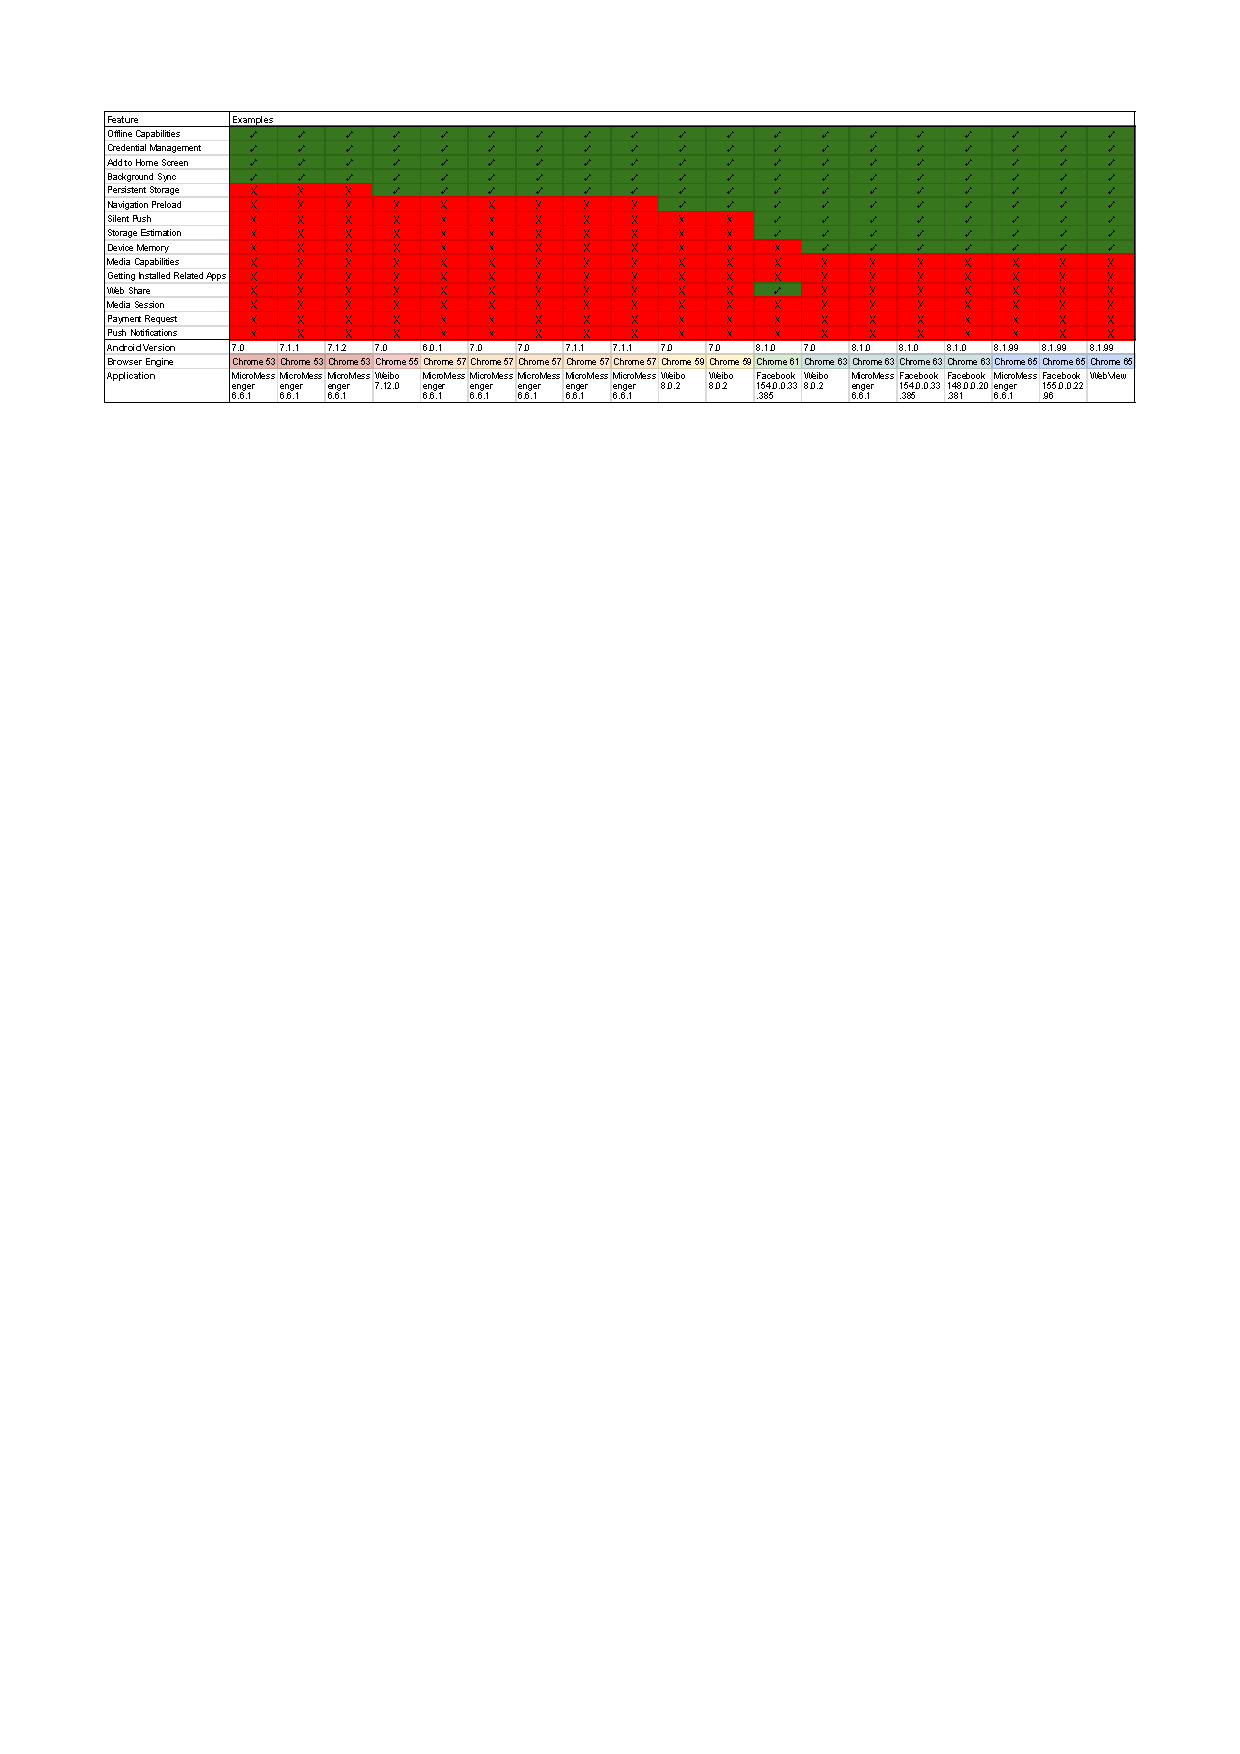
\includegraphics[trim=1.5cm 22.85cm 1.5cm 1.5cm, clip]{webview-results.pdf}}
  % https://docs.google.com/spreadsheets/d/18xaJeIrfaA-8wNucK7IDQMfr5LHjsBcey4lHF3Pkd1o/edit?usp=sharing
  \caption{Increasingly improving \textsc{pwa} feature support situation
    on various Android \texttt{WebView}s, ordered by browser engine and Android version.
    The sole \emph{seemingly} supported Web Share feature in Chrome~61
    was actually a bug (\url{https://crbug.com/765923}).}
  \label{table:webview}
  \end{center}
\end{figure*}

\begin{figure}[t]
  \renewcommand{\figurename}{Table}
  \begin{center}
  \centerline{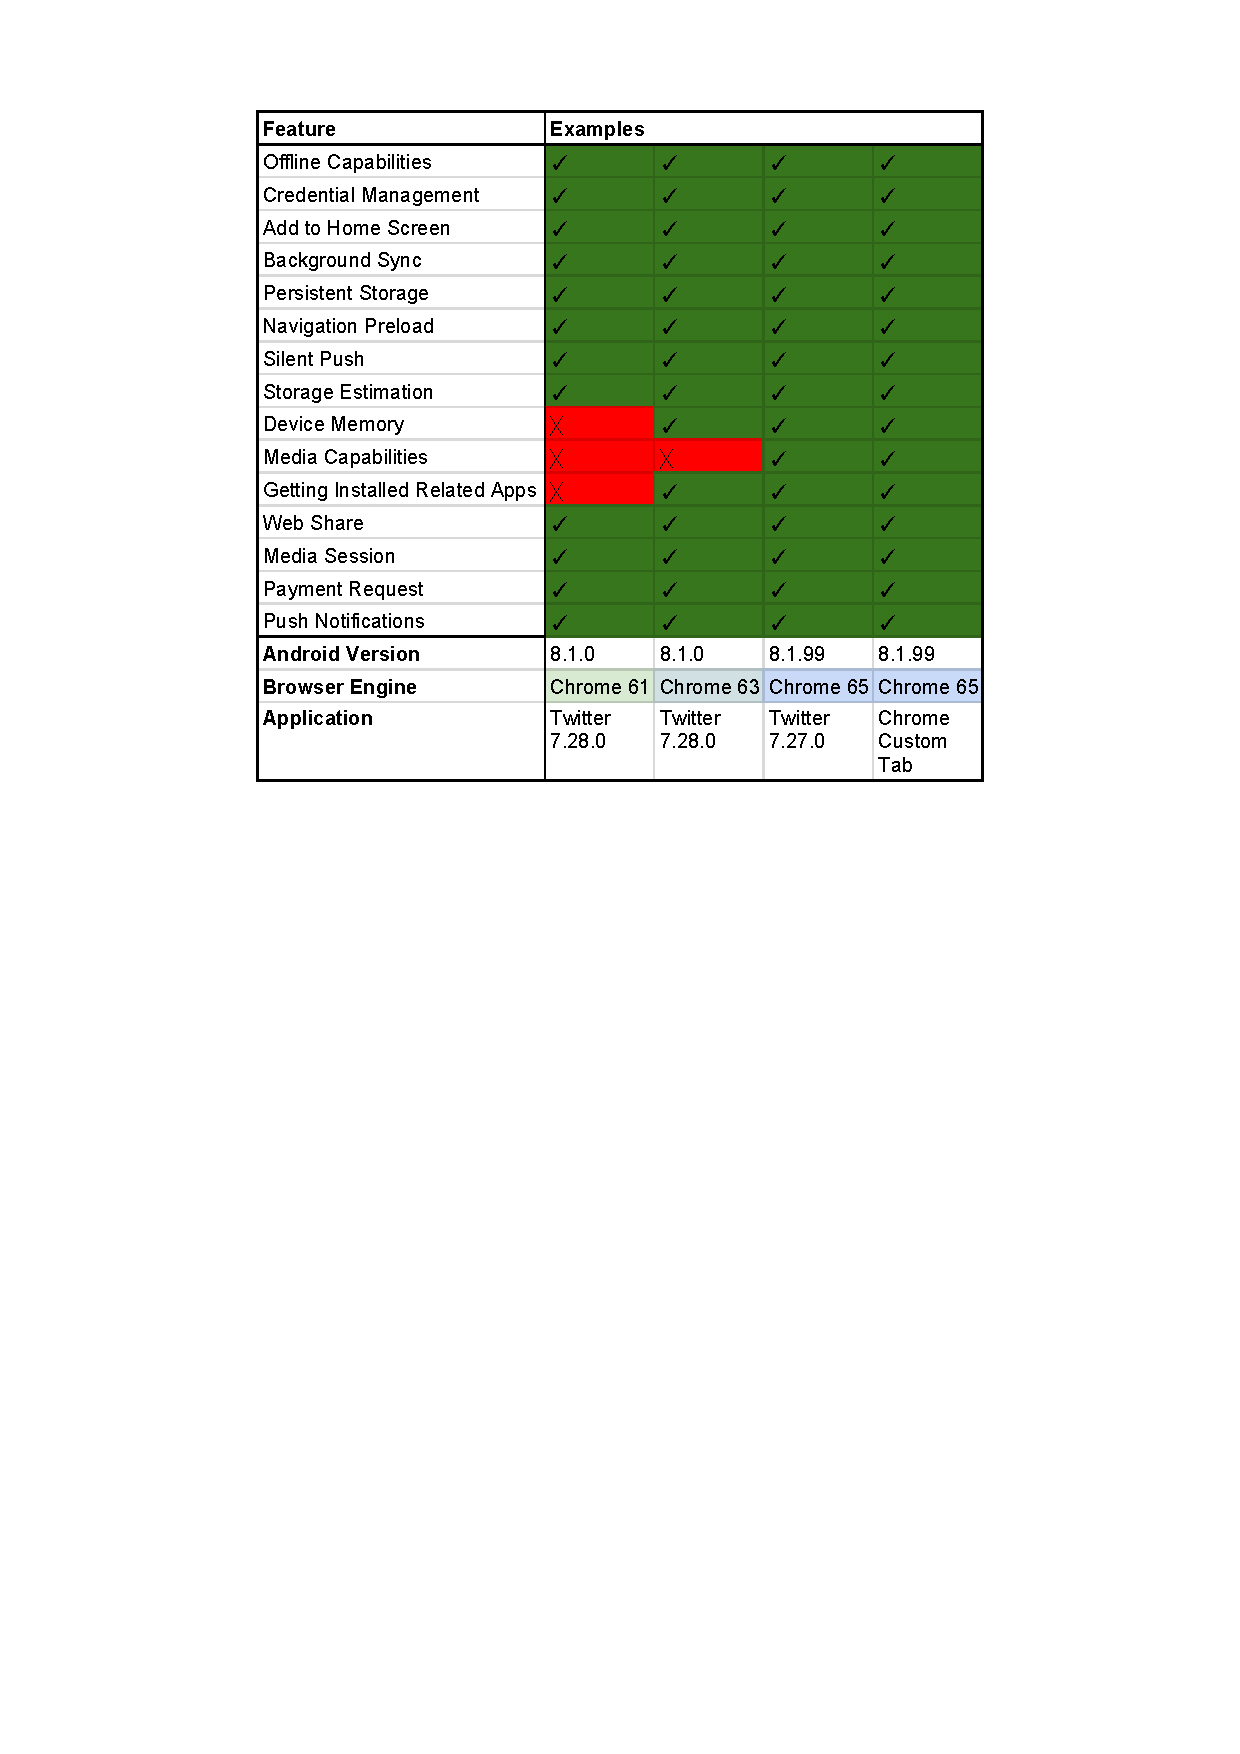
\includegraphics[width=.65\columnwidth,trim=4.3cm 16.4cm 4.3cm 1.5cm, clip]{custom-tab-results.pdf}}
  % https://docs.google.com/spreadsheets/d/18xaJeIrfaA-8wNucK7IDQMfr5LHjsBcey4lHF3Pkd1o/edit?usp=sharing
  \caption{Increasingly improving \textsc{pwa} feature support situation
    on various Android \texttt{CustomTabsIntent}s,
    ordered by browser engine and Android version.}
  \label{table:customtab}
  \end{center}
\end{figure}

\begin{figure}[t]
  \renewcommand{\figurename}{Table}
  \begin{center}
  \centerline{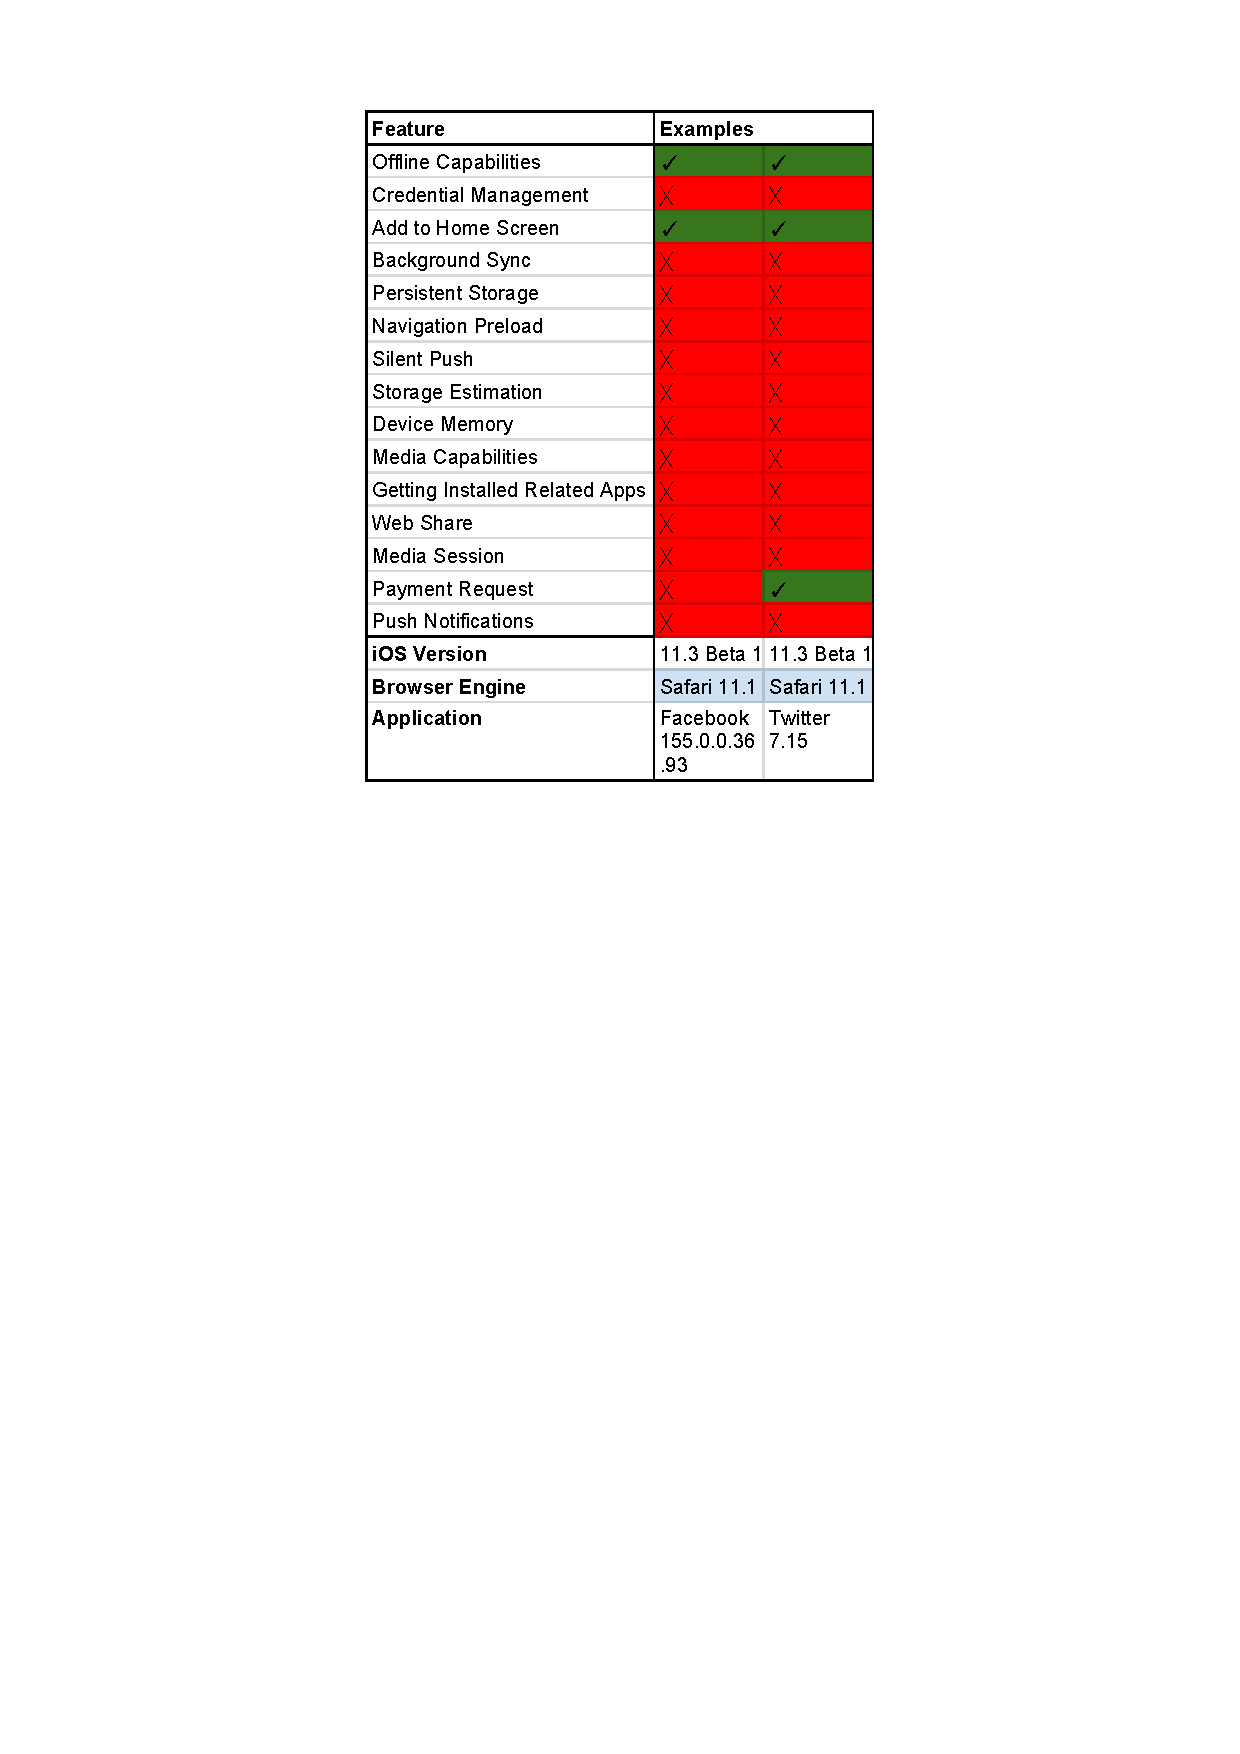
\includegraphics[width=.65\columnwidth,trim=4.3cm 16.4cm 4.3cm 1.5cm, clip]{ios-results.pdf}}
  % https://docs.google.com/spreadsheets/d/18xaJeIrfaA-8wNucK7IDQMfr5LHjsBcey4lHF3Pkd1o/edit?usp=sharing
  \caption{\textsc{pwa} feature support situation on i\textsc{os} for both \texttt{WKWebView} (Facebook)
    and \texttt{CustomTabsIntent} (Twitter).}
  \label{table:safari}
  \end{center}
\end{figure}

\paragraph{Discussion of the \texttt{WebView} Results}

Table~\ref{table:webview} unsurprisingly shows that the more mature
the underlying browser engine gets, the more \textsc{pwa} features become available.
We can see that the \textsc{pwa} features which---according to the feature detection tests
from~\autoref{code:feature-detection}---were reported to be working
from the earliest examined browser engine on are \emph{Offline Capabilities},
\emph{Background Sync}, \emph{Credential Management}, and \emph{Add to Home Screen}.
However, we need to have a~closer look at the results.

\paragraph{\textsc{pwa} Features Reported to Be Working}

\begin{description}
  \itemsep0em 
  \item[Offline Capabilities] Supported from the start, the feature \emph{Offline Capabilities}
    is working as expected.
  \item[Credential Management] The feature \emph{Credential Management}
    is presumably erroneously exposed,
     which is tracked in Chromium bug \url{https://crbug.com/589829}.    
  \item[Add to Home Screen] While in theory supported from the start,
    the situation with \emph{Add to Home Screen} is blurry.
    First, the criteria for \emph{when exactly} the prompt actually triggers
    are not exposed publicly. The conditions listed in~\cite{kinlan2017a2hs} are necessary,
    but not sufficient.
    What the feature test does is check if the browser supports the \texttt{onbeforeinstallprompt} event
    that fires just before a~potential install prompt would be shown,
    and whether it knows how to deal
    with a~Web App Manifest.
    However, if it then actually shows a~prompt
    is left to browser implementers~\cite{caceres2017manifest}.
  \item[Background Sync] While in theory supported from the start,
    \emph{Background Sync} exists, but fails upon trying to use it.
    This is tracked in Chromium bug \url{https://crbug.com/570713}.
  \item[Persistent Storage] Chrome~55 added support for
     \emph{Persistent Storage}~\cite{vankesteren2018storage},
     but while the \texttt{navigator.storage.persist} method exists and can be called,
     the result is always negative, so data is actually never persisted.
  \item[Navigation Preload] The feature \emph{Navigation Preload}, added in Chrome~59
    is working as expected.
  \item[Silent Push] \emph{Silent Push}, added in Chrome~61 has a~method
    \texttt{navigator.budget.reserve} that returns nothing, where a~boolean value is expected.
    Like \emph{Push Notifications} it is not supposed to work.
  \item[Storage Estimation] The feature \emph{Storage Estimation}, added in Chrome~61,
    is working as expected.
  \item[Device Memory] The feature \emph{Device Memory}, added in Chrome version~63, 
    is working as intended.
  \item[Web Share] The \emph{Web Share} feature, introduced in Chrome~61,
    was for this one version of Chrome reported to be working, but fixed
    to be no longer exposed in the browser via Chromium bug \url{https://crbug.com/765923}.
\end{description} 

\paragraph{\textsc{pwa} Features Reported Not to Be Working}

\begin{description}
  \item[Push Notifications] The feature \emph{Push Notifications} is supposed and confirmed not to be working.
  \item[Payment Request] The feature \emph{Payment Request} is supposed and confirmed not to be working.
  \item[Media Session] The feature \emph{Media Session} is confirmed not to be working,
    it might be enabled in the future, though, as discussed in Chromium bug
    \url{https://crbug.com/678979}.
  \item[Media Capabilities] The feature \emph{Media Capabilities} is confirmed not to be working,
    it might be enabled in the future, though, as discussed in Chromium bug
    \url{https://crbug.com/690364}.
  \item[Getting Installed Related Apps] The feature \emph{Getting Installed Related Apps}
    is supposed and confirmed not to be working.
\end{description} 

\paragraph{Discussion of the \texttt{CustomTabsIntent} Results}

The results in Table~\ref{table:customtab} present no surprises. 
We can see \emph{Device Memory} support and \emph{Getting Installed Related Apps} support
be added in Chrome~63, and \emph{Media Capabilities} in Chrome~65.
Everything else is confirmed to be working as intended,
as \texttt{CustomTabsIntent} is as close to the system browser as it gets,
like outlined in \autoref{sec:background}.

Regarding \texttt{TrustedWebUtils},
the results are exactly the same as with \texttt{CustomTabsIntent},
because \texttt{TrustedWebUtils} internally just launches a~\texttt{CustomTabsIntent}
and sets a~special flag called \texttt{EXTRA\_LAUNCH\_AS\_TRUSTED\_WEB\_ACTIVITY}.

\subsection{i\textsc{os}}

We have run \textsc{pwa} Feature Detector on Beta versions of i\textsc{os}~11.3,
the first operating system by Apple that ships with a~\textsc{pwa}-capable browser.
Table~\ref{table:safari} shows the very limited set of \textsc{pwa} features
that are available so far on \texttt{WKWebView} and \texttt{SFSafariViewController}.
Albeit Apple made no official announcement of the newly-gained Service Worker support,
Safari Engineer Mondello's tweet~\cite{mondello2018safari} was widely shared and favorited,
proving how eagerly awaited Apple's buy-in was in the broader \textsc{pwa} community.

\paragraph{\textsc{pwa} Features Reported to Be Working}

\begin{description}
  \itemsep0em 
  \item[Offline Capabilities] While some bugs
    exist,\footnote{\url{https://bugs.webkit.org/buglist.cgi?component=Service\%20Workers&list_id=3439423&product=WebKit&resolution=---}} the feature \emph{Offline Capabilities}
    is working as expected on both \texttt{WKWebView} and \texttt{SFSafariViewController}.
  \item[Add to Home Screen] The browser is confirmed~\cite{mondello2018safari}
    to make use of the information in the Web App Manifest,
    but no automatic prompting to install applications happens.
    The corresponding \texttt{onbeforeinstallprompt} event is missing.
    As no prompt is being shown, and the manual ``Add to Home Screen'' functionality
    is only exposed in stand-alone Safari, neither \texttt{SFSafariViewController} nor \texttt{WKWebView}
    actually support add to home screen.
  \item[Payment Request] The feature \emph{Payment Request} is supposed
    to be working on \texttt{SFSafariViewController}, but calling the \texttt{paymentRequest.canMakePayment()}
    method always returns a~negative result.
\end{description} 

\paragraph{\textsc{pwa} Features Reported Not to Be Working}

All other \textsc{pwa} features are supposed and confirmed not to be working.

\begin{figure}[h]
  \centering
  \begin{subfigure}[t]{0.475\columnwidth}
    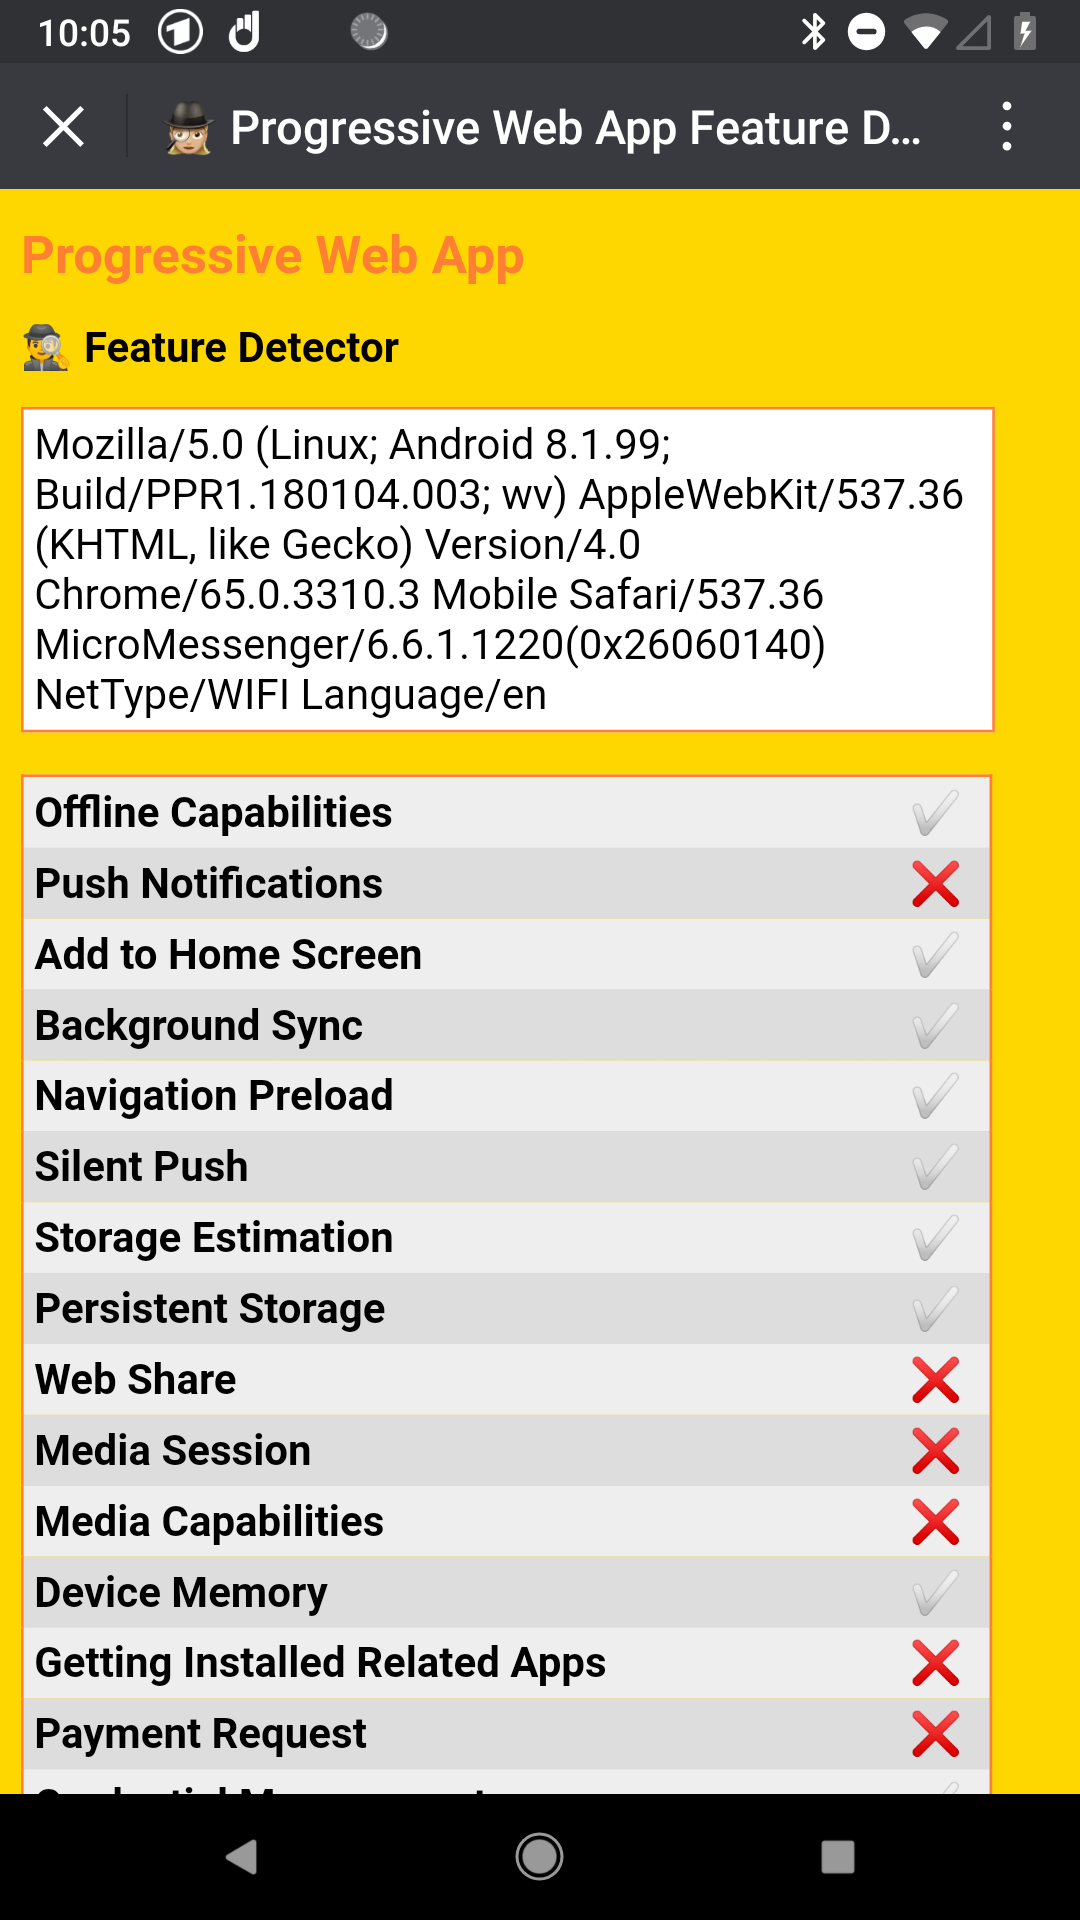
\includegraphics[width=1\columnwidth,frame]{pwa-feature-detector-wechat-android-chrome65}
    \caption[\textsc{pwa} Feature Detector running in WeChat.]{
      In WeChat in a~Chrome~65 based \texttt{WebView}.}
    \label{fig:wechat-android-chrome65}
  \end{subfigure}    
  \quad
  \begin{subfigure}[t]{0.475\columnwidth}  
    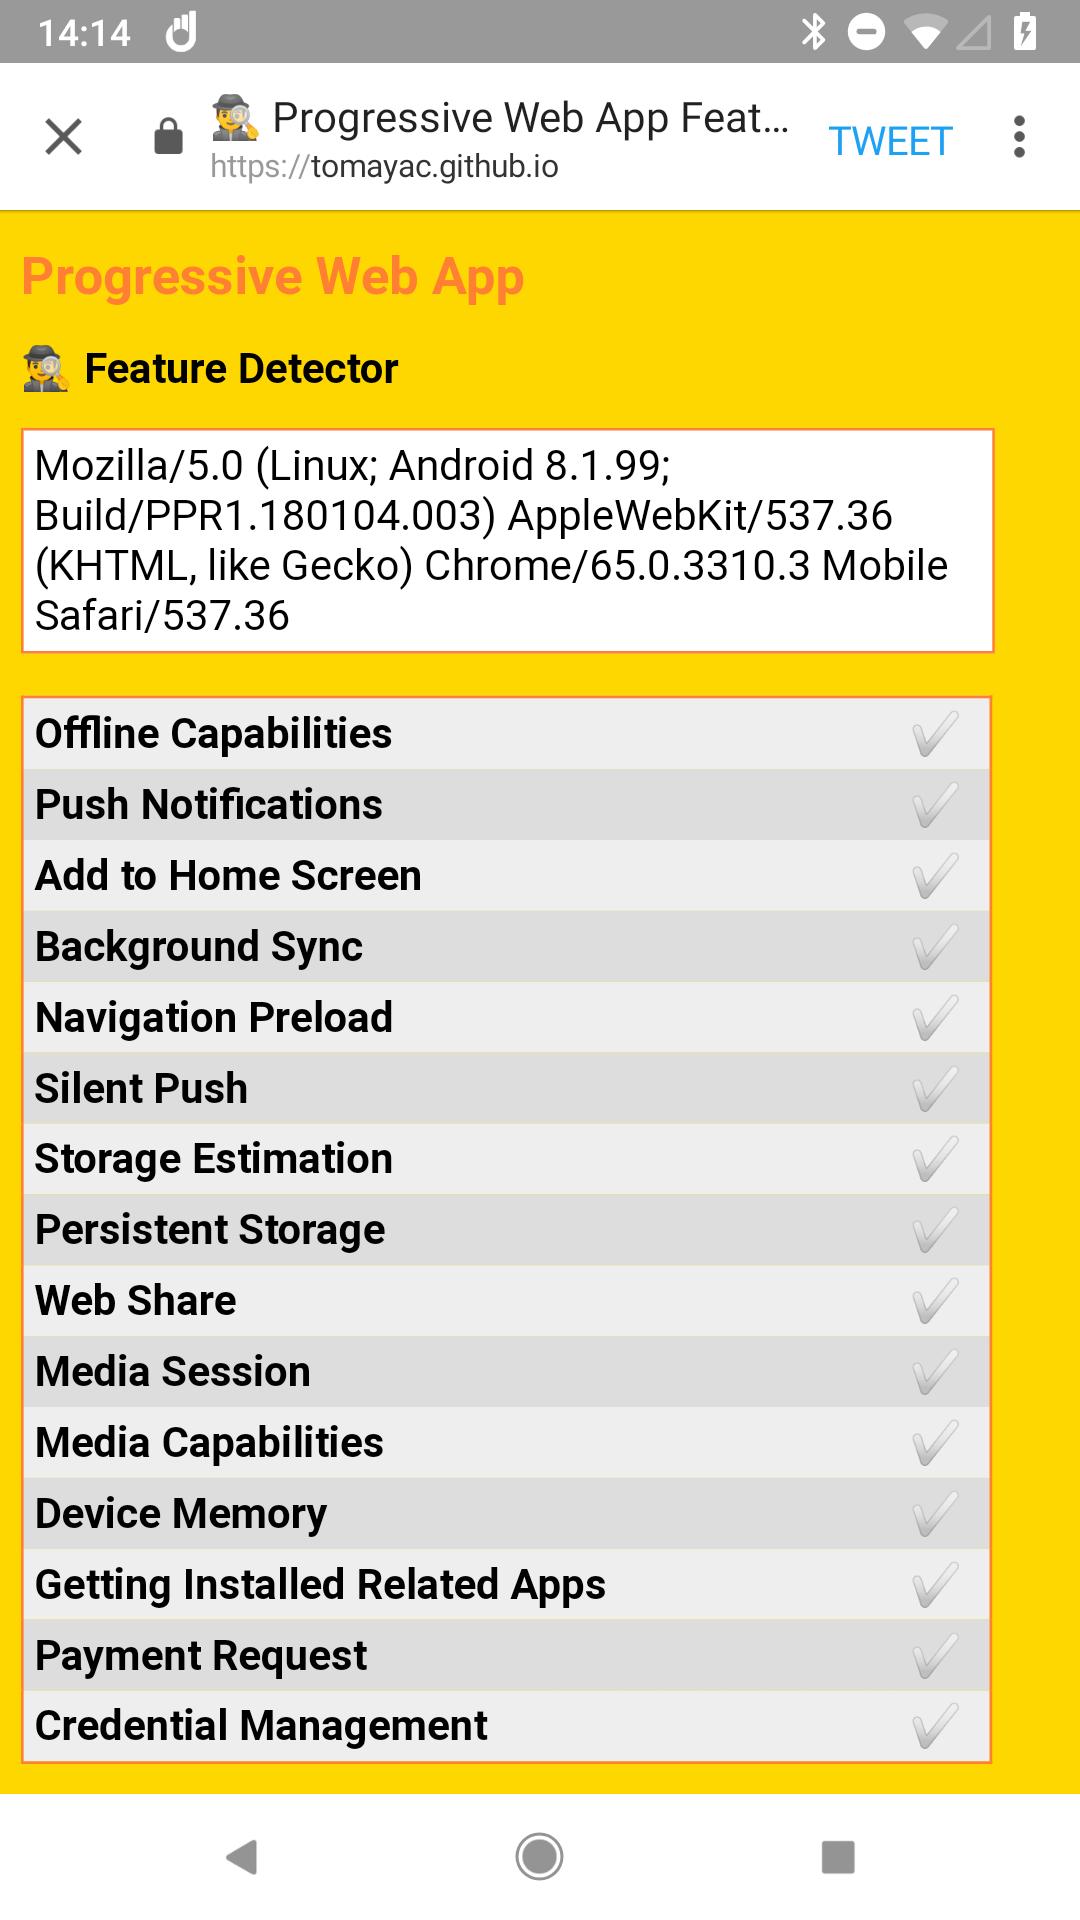
\includegraphics[width=1\columnwidth,frame]{pwa-feature-detector-twitter-android-chrome65}
    \caption[\textsc{pwa} Feature Detector running in Twitter.]{
      In Twitter in a~Chrome~65 based \texttt{CustomTabsIntent}.}
    \label{fig:twitter-android-chrome65}
  \end{subfigure}
  \caption{\textsc{pwa} Feature Detector running on Android~8.1.99.}    
\end{figure}

\begin{figure}[h]
  \centering
  \begin{subfigure}[t]{0.475\columnwidth}
    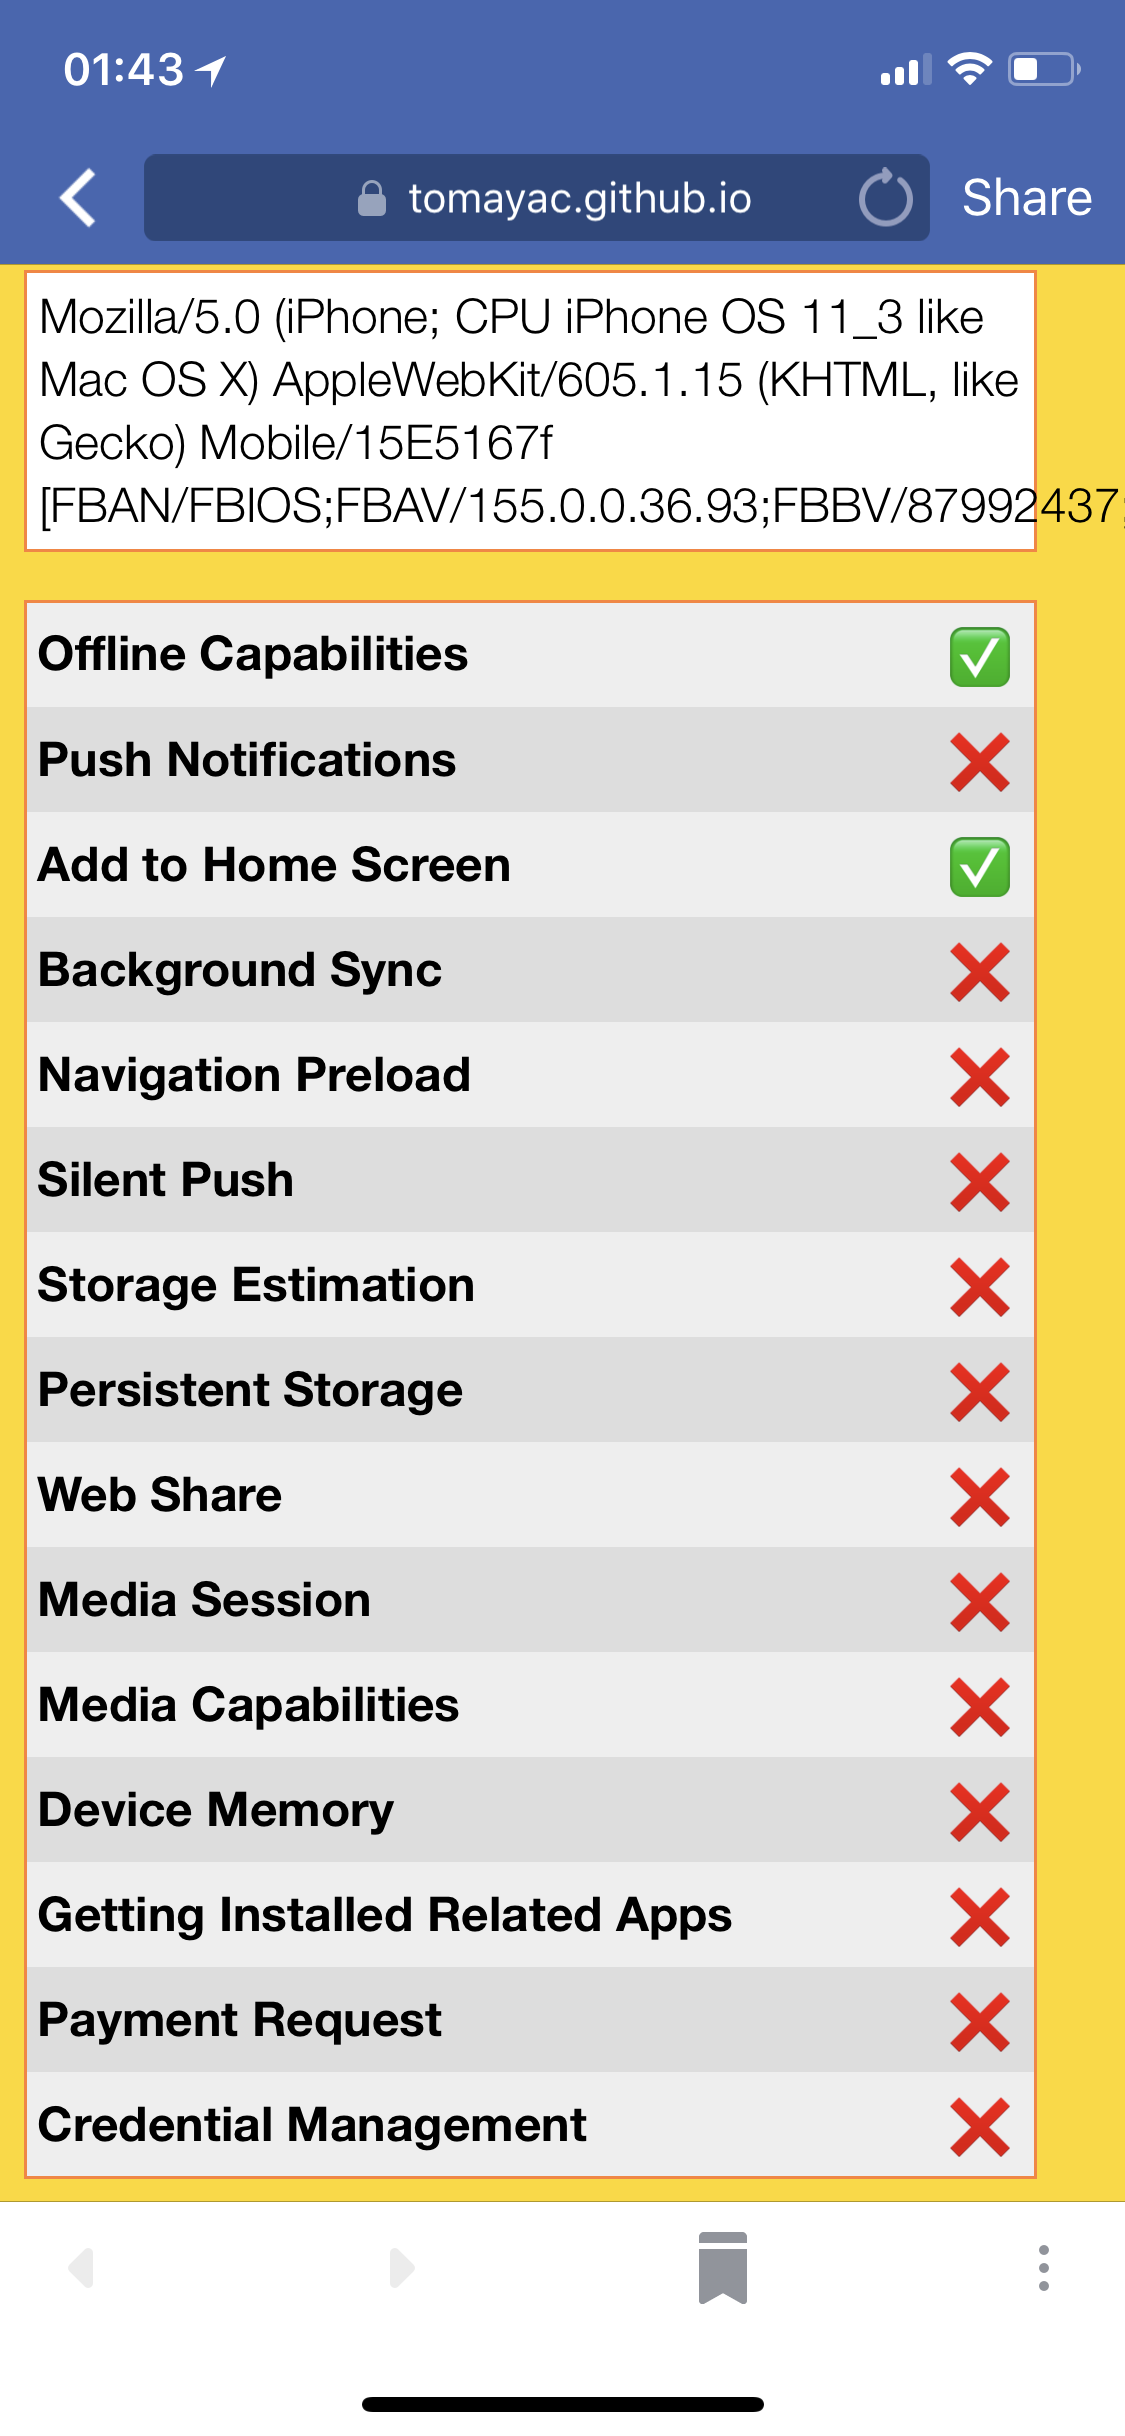
\includegraphics[width=1\columnwidth,frame]{pwa-feature-detector-facebook-ios-safari11_1}
    \caption[\textsc{pwa} Feature Detector running in Facebook.]{
      In Facebook in a~Safari~11.1 based \texttt{WKWebView}.}
    \label{fig:facebook-ios-safari11_1}
  \end{subfigure}    
  \quad
  \begin{subfigure}[t]{0.475\columnwidth}  
    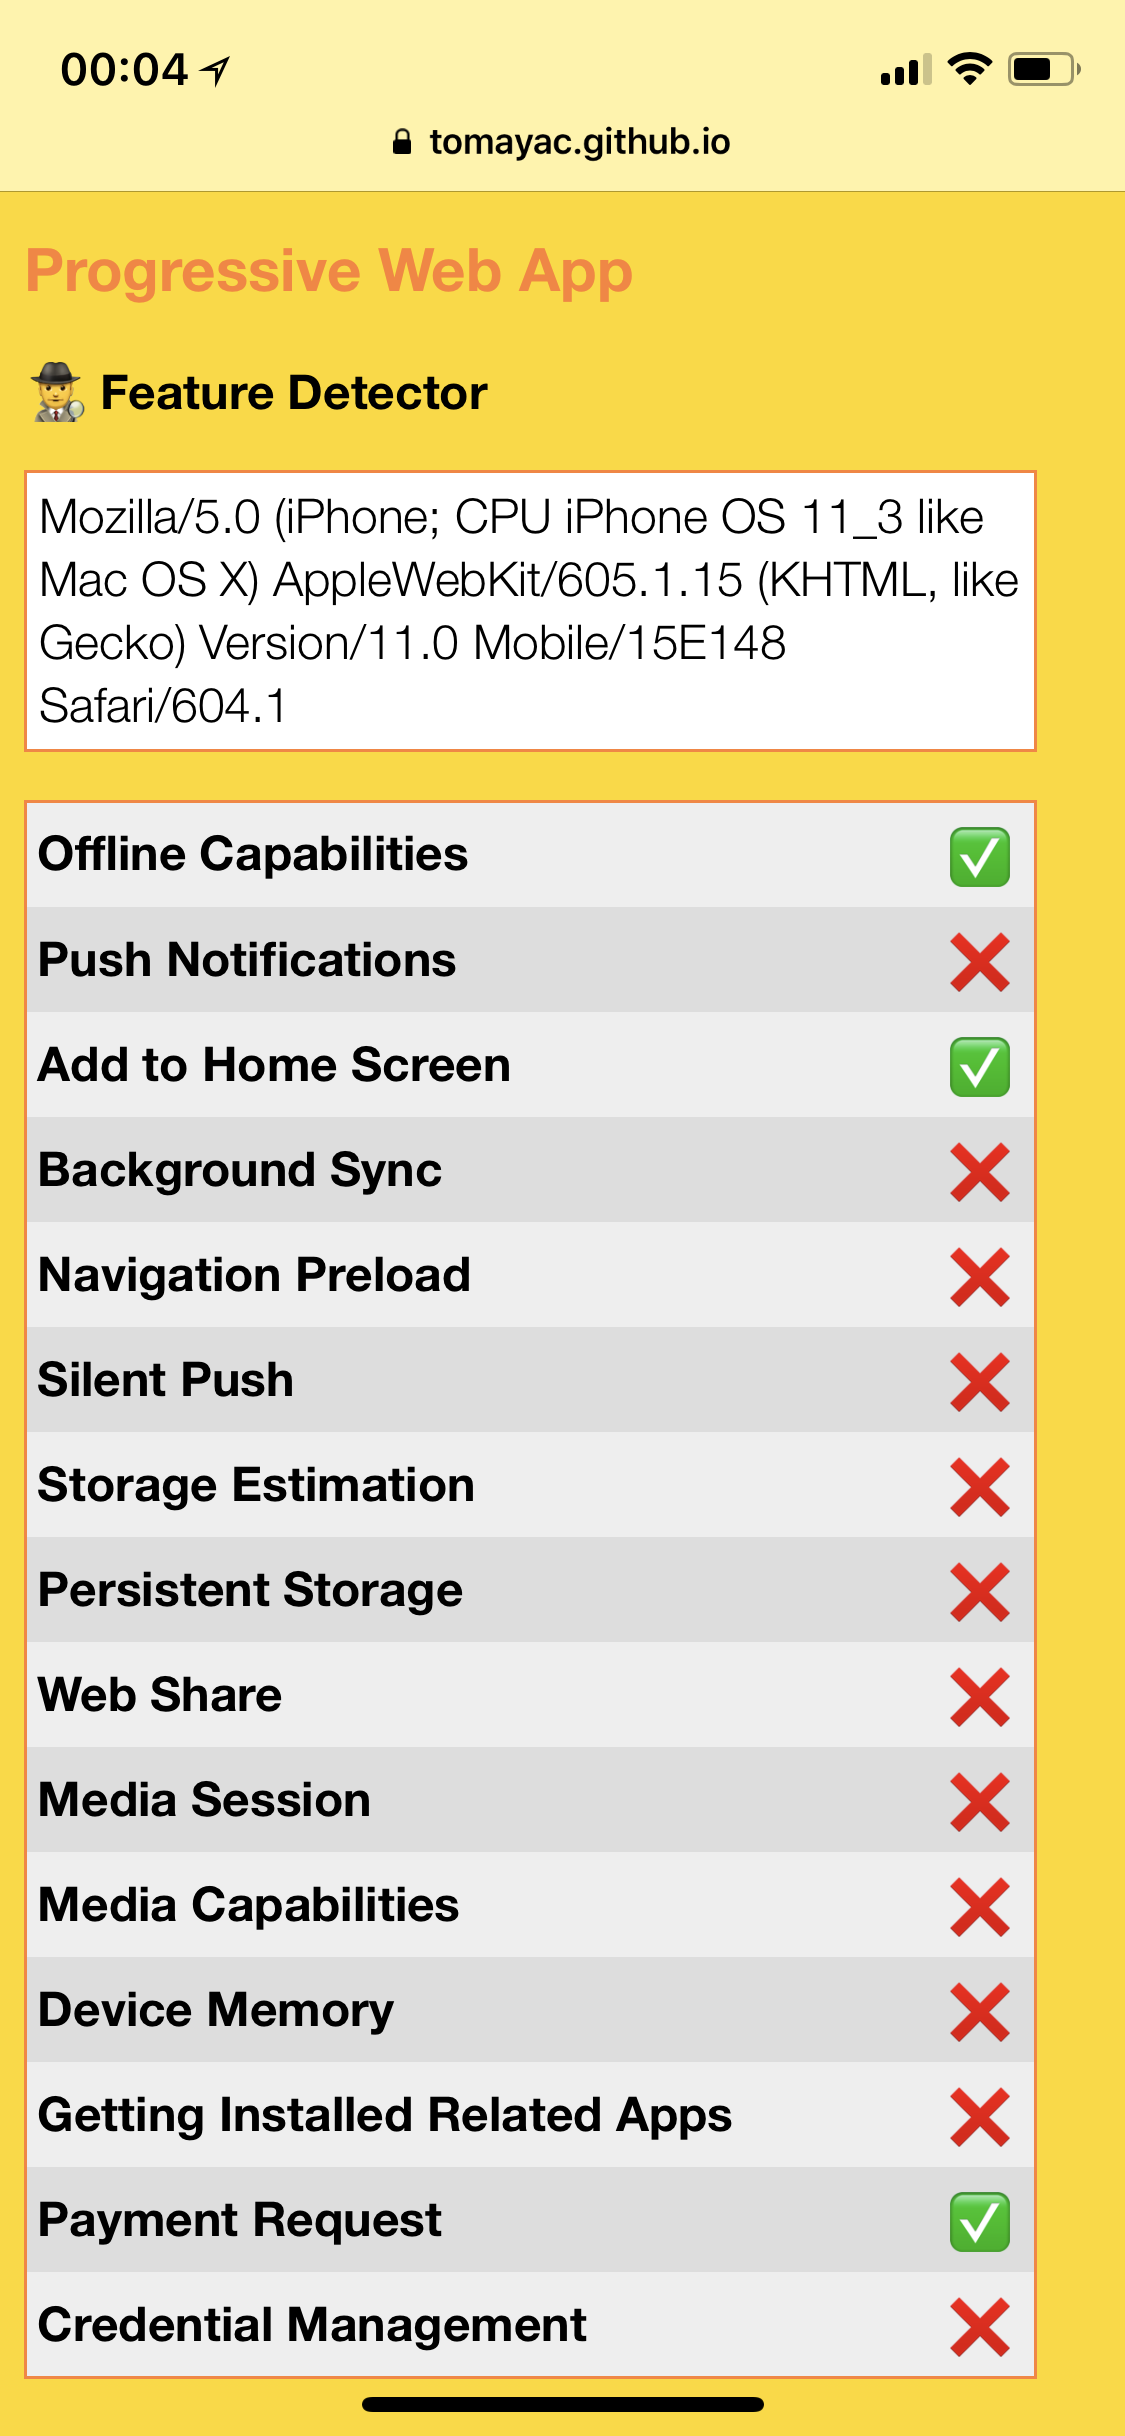
\includegraphics[width=1\columnwidth,frame]{pwa-feature-detector-twitter-ios-safari11_1}
    \caption[\textsc{pwa} Feature Detector running in Twitter.]{
      In Twitter in a~Safari~11.1 based \texttt{SFSafariViewController}.}
    \label{fig:twitter-ios-safari11_1}
  \end{subfigure} 
  \caption{\textsc{pwa} Feature Detector running on i\textsc{os}~11.3 Beta~1.}       
\end{figure}

\section{Future Work}
\label{sec:future-work}

Future work will cover two aspects:
we look at it from the point of view of app developers
programming \textsc{pwa}s for Web Views,
as well as from the angle of a~browser vendor.

\subsection{Improving Feature Tests}

First, we will look into improving the feature detection tests in
\autoref{code:feature-detection}.
Such tests always need to be side-effect-free,
so in the majority of cases naively trying to execute an exposed method
rather than just testing for its existence is prohibitive.
We have seen that no-op or dummy methods like with \emph{Silent Push},
where \texttt{navigator.budget.reserve} just did nothing,
or with \emph{Persistent Storage}, 
where the method \texttt{navigator.storage.persist} always returned a~negative response
can be the reason for unexpected results.
In an ideal world, existence tests should just be good enough,
which requires catching involuntarily exposed interfaces.
Chromium bug \url{https://crbug.com/787868} has as an objective
to automatically identify such cases.

\subsection{Polyfilling Missing \textsc{api}s in \texttt{WebView}s}

While generally \texttt{CustomTabsIntent} is the Web View of choice,
there may be reasons where app developers are stuck with \texttt{WebView}.
A~\emph{polyfill} is code that implements a~feature on Web browsers
that do not support the feature.
The \texttt{WebView.evaluateJavascript} method allows JavaScript code to be 
asynchronously evaluated in the context of the currently displayed page.
For app developers, this can help improve
the \textsc{pwa} support situation for some \textsc{api}s
that can, at least to some extent, be polyfilled.
One example might be \emph{Push Notifications},
albeit polyfills like \texttt{notification.js}\footnote{\url{https://adodson.com/notification.js/}} 
can acknowledgedly only partially work due to technical constraints.

\section{Conclusions}
\label{sec:conclusions}

In this paper, we have first provided the technical background on Web Views
on both Android and i\textsc{os}.
Second, we have defined a~number of \textsc{pwa} features
and documented and implemented tests for detecting them
in the open source app \textsc{pwa} Feature Detector. 
In continuation, we have evaluated the approach on a~great variety of devices
with different versions of operating systems, Web Views,
and applications with in-app browser.
We have identified a~number of issues with these feature tests,
and have collected various interfaces that are exposed erroneously in browsers.

\todo{Write Conclusions}

\section*{Acknowledgements}

\emph{Alex Russell}'s review comments have greatly helped sharpen the points made in this paper.
We would like to thank the \emph{participants of the Google Developer Days~2017 in Shanghai, China},
who helped gather the statistical data and sent us
the screenshots on WeChat.
Further, we would like to thank \emph{Adam Bar} of \url{https://whatwebcando.today} fame
for the helpful discussions around feature detection.

\begin{figure*}[b]
  \begin{center}
  \centerline{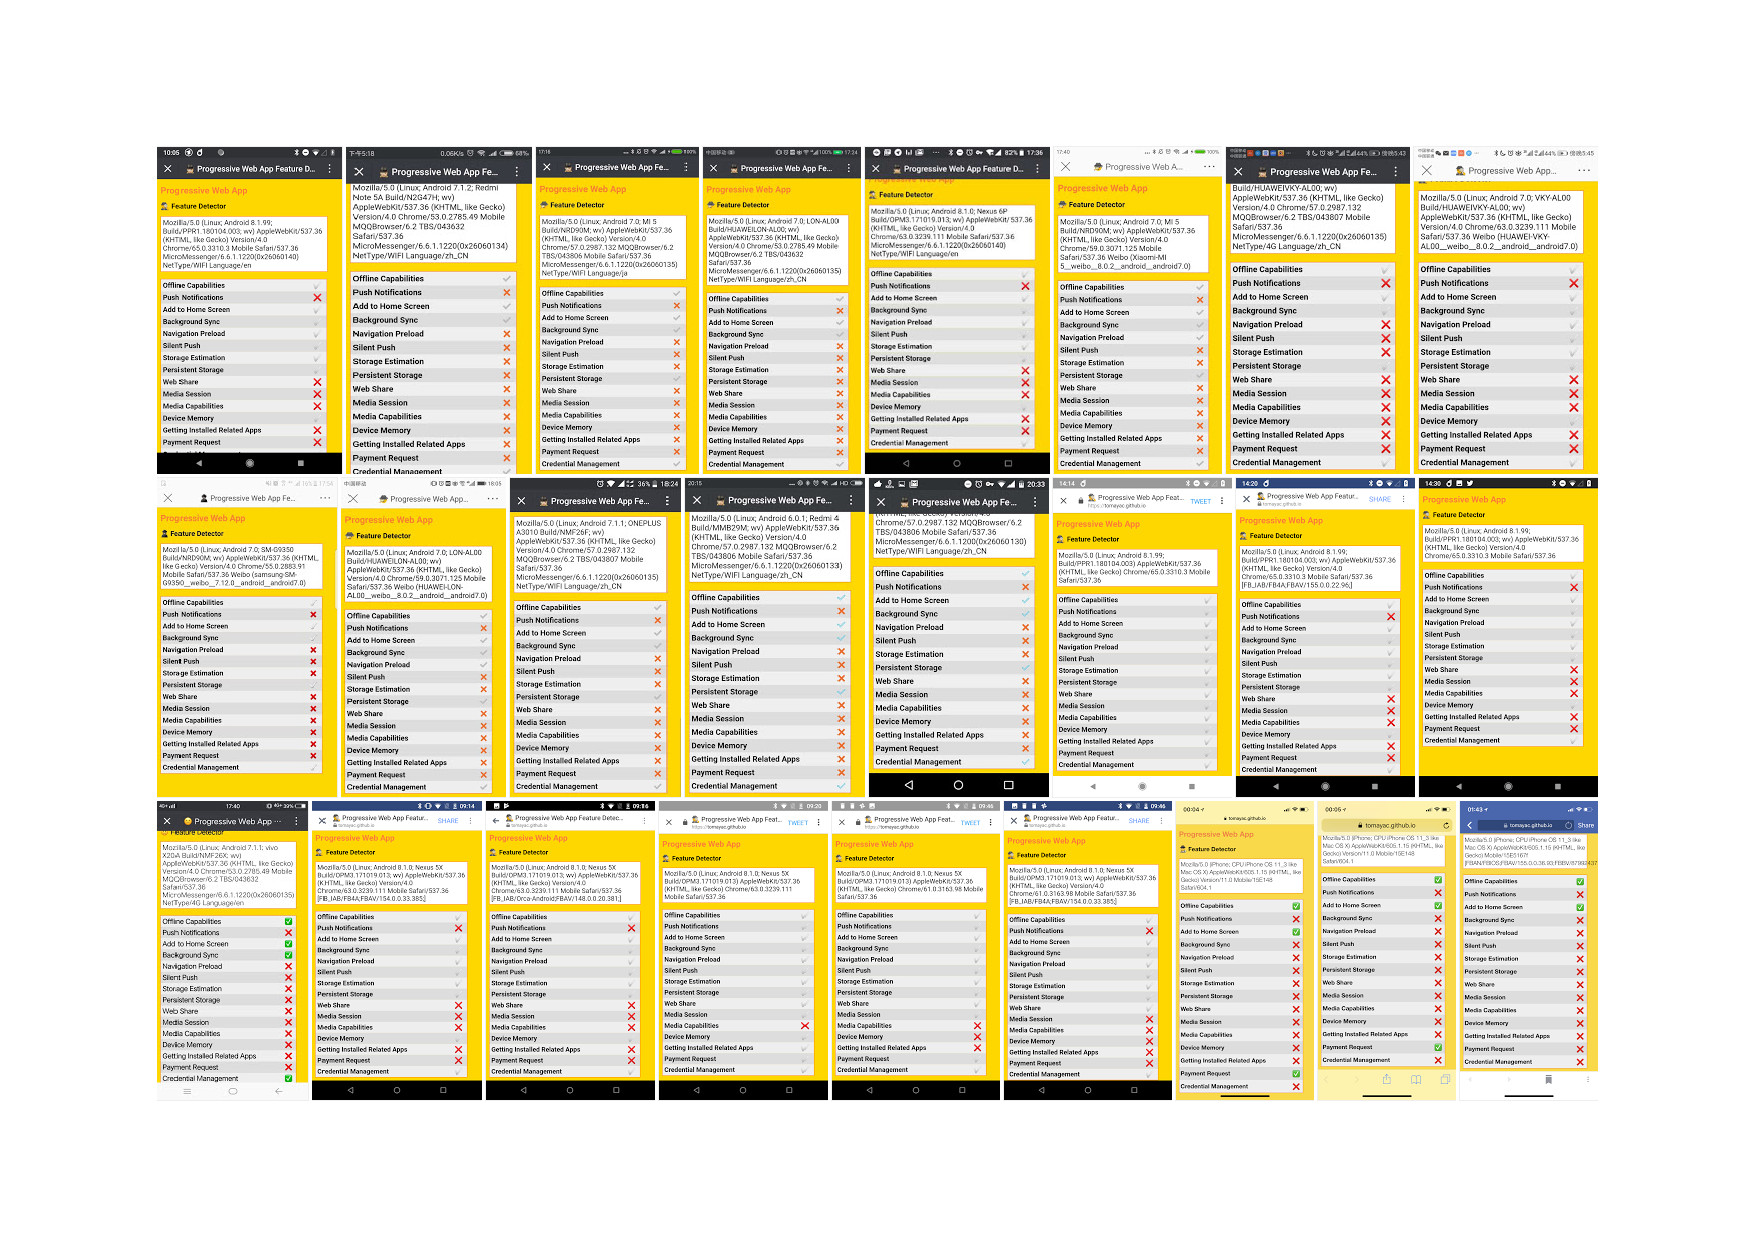
\includegraphics[width=\paperwidth, trim=0cm 2.5cm 0cm 0cm, clip]{index-sheet.pdf}}
  \caption{Index sheet with all tested device screenshots showing Android \texttt{WebView}s and
    \texttt{CustomTabsIntent}s, as well as i\textsc{os} \texttt{WKWebView} and \texttt{SFSafariViewController},
    running in different applications.
    Higher resolution screenshots are available at \url{https://photos.app.goo.gl/Kh3DyhpL6Q58G7tn1}.}
  \label{fig:indexsheet}
  \end{center}
\end{figure*}

\bibliographystyle{ACM-Reference-Format}
\bibliography{bibliography}

\end{document}
